\section{Self-Suspending Tasks in Multiprocessor Synchronizations}
\label{sec:syn}

In this section, we consider multiprocessors subject to \emph{partitioned fixed-priority (\pfp)} scheduling, and review the general analysis strategies for tasks that synchronize access to shared resources (\eg, shared I/O devices, communication buffers, or scheduler locks) with suspension-based locks (\eg, binary semaphores). Unfortunately, some of the misconceptions surrounding the analysis of self-suspensions on uniprocessors also spread to the analysis of partitioned multiprocessor real-time locking protocols. In particular, as we show with a counterexample, the analysis framework to account for the additional interference due to \emph{remote blocking} first introduced in \cite{lakshmanan-2009}, and reused in several other works~\cite{zeng-2011,bbb-2013,yang-2013,kim-2014,han-2014,carminati-2014,yang-2014},  is flawed. Finally, a straightforward solution for these problems are discussed. 

\subsection{Existing analysis strategies}
\label{sec:papers}

\pfp scheduling is a widespread choice in practice due to the wide support in industrial standards such as AUTOSAR, and in many RTOSs like VxWorks, RTEMS, ThreadX, \etc Under \pfp scheduling, each task has a fixed base priority and is statically assigned to a specific processor, and the tasks on each processors are scheduled as in uniprocessors. 

\iffalse
At runtime, a resource-holding job may be assigned a temporarily elevated effective priority according to the employed locking protocol. Thus on each processor, the ready job with highest effective priority is scheduled.\todo{Why are effective priorities relevant here? Just cut it?} 
\fi

Under partitioned scheduling, a resource accessed by tasks from different processors is called a \emph{global resource}, otherwise it is called a \emph{local resource}. When a job requests a global resource, it may incur \emph{remote blocking} if the global resource is held by a job on another processor. Also, a job may incur \emph{local blocking} if it is prevented from being scheduled by a resource-holding job of a lower-priority task on its local processor. 

Under suspension-based protocols, such as the \emph{multiprocessor priority ceiling protocol (MPCP)}~\cite{rajkumar-1990}, tasks that are denied to access shared resources are suspended. From the perspective of local schedule on each processor, remote blocking, caused by external events (\ie, resource contention due to tasks on the other processors), pushes the execution of higher-priority tasks to a later time point regardless of the schedule on the local processor (\ie, even if the local processor is idle), thus may cause additional interference on lower-priority tasks. To this end, remote blocking is considered as self-suspension in analysis. Whereas, local blocking takes place only if a local lower-priority task is scheduled (\ie, the local processor is busy). Consequently, local blocking is accounted for as regular blocking as in uniprocessors, but not as self-suspension.

In analysis, a safe yet pessimistic strategy is to convert remote blocking into computation. Accordingly, the remote blocking incurred by each higher-priority task is counted as part of interference. \citet{block-2007} first used this strategy for partitioned \emph{earliest deadline first (EDF)} scheduling;  \citet{lakshmanan-2009} also adopted this approach in their analysis of ``virtual spinning,'' where when a task is suspended due to remote blocking other tasks are allowed to execute unless they try to access global resources. An alternative is to bound the effects of deferred execution due to remote blocking. Recently, \citet{lakshmanan-2009} proposed the following response-time analysis framework that takes into account the amount of remote blocking to bound the worst case interference.

\begin{align}
\label{eq:wcrt}
R_k^{n+1} = C_k^{\star} + \sum_{\tau_i \in \fun{hp(k)} \cap P(\tau_k)} \left \lceil \frac{R_k^n + B_i^r}{T_i} \right \rceil \cdot C_i + s_k \sum_{\tau_l \in \fun{lp(k)} \cap P(\tau_k)} \max_{1 \leq j < s_l} C_{l,j}^{\prime}.  
\end{align}
where $C_k^{\star} = C_k + B_k^r$, $R_k^0 = C_k^{\star}$, and $\tau_k$ is considered schedulable if $R_k^{n+1} = R_k^n < D_k$. 

In \equref{wcrt}, $B_k^r$ is an upper bound on the maximum remote blocking that a job of $\tau_k$ incurs. $\fun{hp(k)}$ and $\fun{lp(k)}$ denote the tasks with higher and lower priority than $\tau_k$, respectively. $P(\tau_k)$ denotes the tasks that are assigned on the same processor as $\tau_k$. $s_k$ is the maximum number of critical sections of $\tau_k$. $C_{l,j}^{\prime}$ is an upper bound on the execution time of the $j$th critical section of $\tau_l$. The additional interference on $\tau_k$ due to the remote blocking incurred by each higher-priority task is captured in the analysis according to the second term in \equref{wcrt}.

Under this analysis framework, $\left \lceil \frac{R_k + B_i^r}{T_i} \right \rceil \cdot C_i$ is used as an upper bound on the total interference of $\tau_i$ on $\tau_k$. This analysis approach was reused in \cite{yang-2013,kim-2014,carminati-2014,yang-2014} to analyze (several variants of) the \mpcp. The response-time analysis framework (\ie, \equref{wcrt}) was also reused in \cite{zeng-2011,bbb-2013,han-2014} to compare the schedulability performances between different locking protocols under \pfp scheduling. 

Unfortunately, the analysis approach based on \equref{wcrt} fails to guarantee a safe response time bound in certain corner cases, as can be demonstrated with the following counterexample.

\subsection{A counterexample}
\label{sec:counterexample}

We show the existence of a schedule in which a task that is considered schedulable according to the analysis in \cite{lakshmanan-2009} is in fact unschedulable.

\begin{figure}[!ht]
\captionsetup{belowskip=-1pt}
\begin{center}
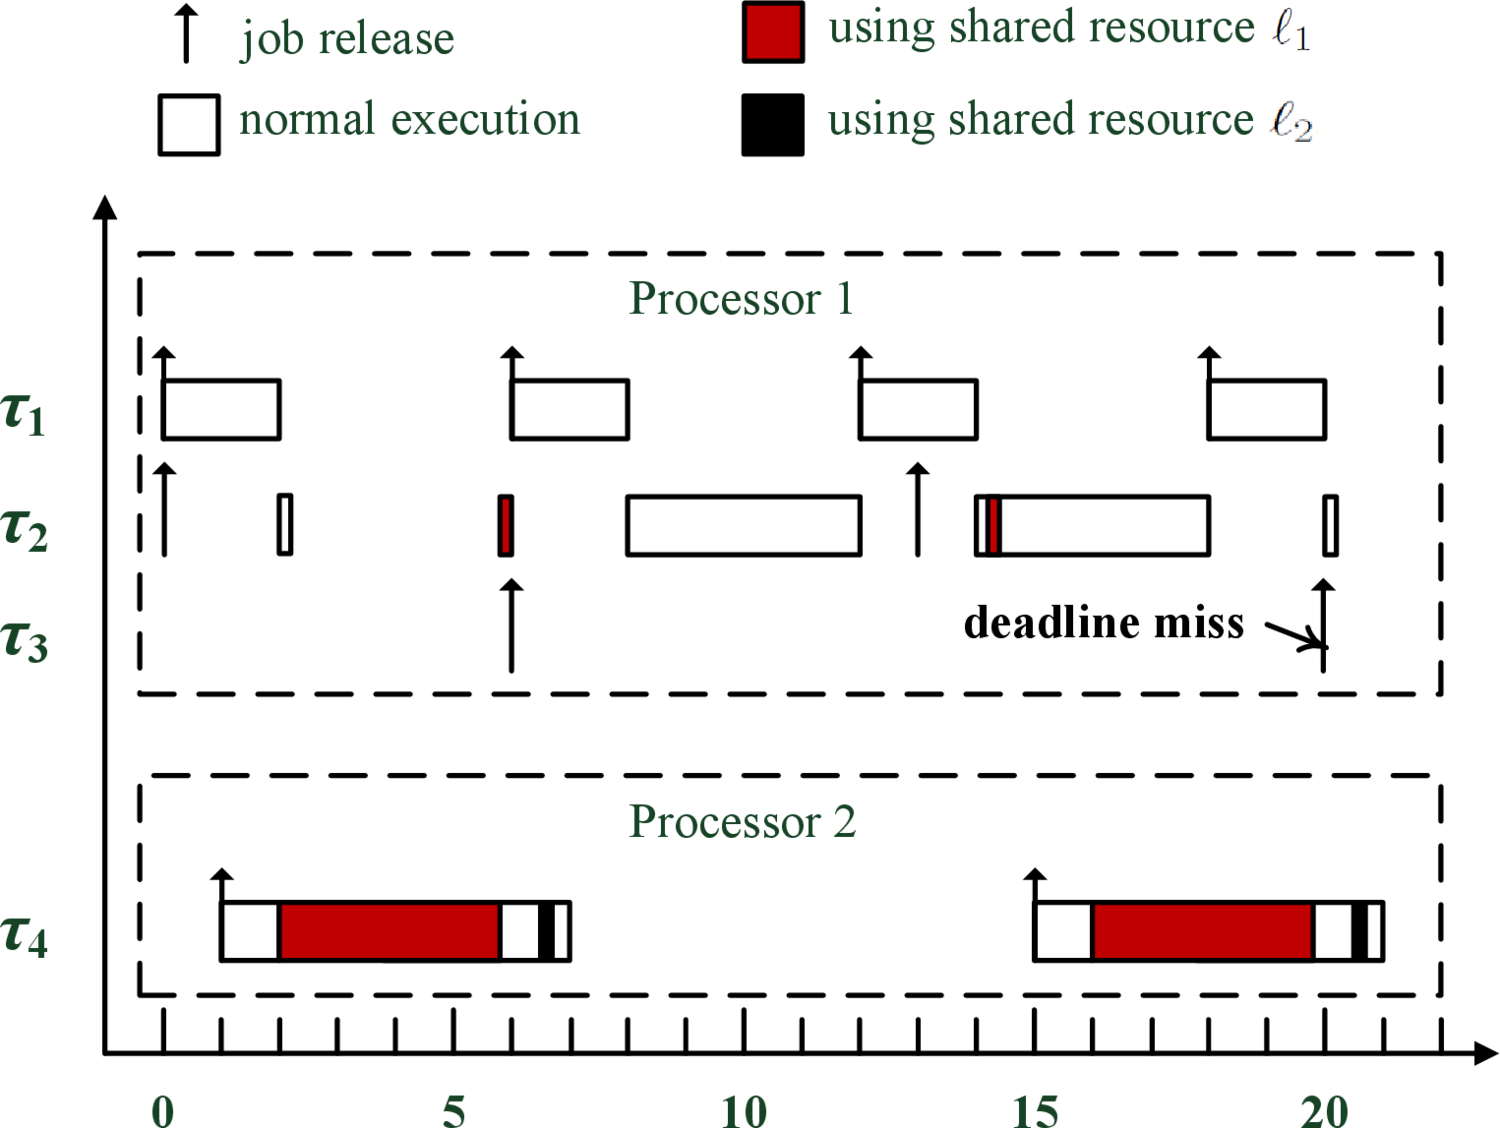
\includegraphics[width=12cm]{Counterexample}
\caption{An example schedule in which the first job of $\tau_3$ misses its deadline. 
}
\label{fig:counterexample}
\end{center}
\end{figure}

\input{parameters}

Consider four implicit deadline sporadic tasks ${\tau_1, \tau_2, \tau_3, \tau_4}$ (with parameters listed in \tabref{parameters}, where $N_{k,1}$ ($N_{k,2}$) denotes the maximum number of requests that a job of $\tau_k$ can issue to resource $\res_1$ ($\res_2$), and $L_{k,1}$ ($L_{k,2}$) denotes the corresponding maximum critical section length), ordered by decreasing order of priority, that are scheduled on two processors using \pfp scheduling. $\tau_1$, $\tau_2$ and $\tau_3$ are assigned to processor 1, while $T_4$ is assigned to processor 2. Jobs of $\tau_2$ and $\tau_4$   each once access a shared resource $\res_1$  ($N_{2,1} = 1$ and $N_{4,1} = 1$). Jobs of $\tau_4$ each once access a shared resource $\res_2$ ($N_{4,2} = 1$). Each job of $\tau_2$ uses $\res_1$ for a duration of at most $L_{2,1} = \varepsilon < 1$ time units (an arbitrarily small quantity), and each job of $\tau_4$ uses $\res_1$ and $\res_2$ for at most $L_{4,1} = 4-\varepsilon$ and $L_{4,1} = \varepsilon$ time units respectively. 

Consider the response-time of $\tau_3$. Since $\tau_3$ is the lowest-priority task on its processor, it does not incur any local blocking (\ie,$s_3 \sum_{\tau_l \in \fun{lp}(3) \cap P(\tau_3)} \max_{1 \leq j < s_l} C_{l,j}^{\prime} = 0$). While each time $\tau_3$ requests $\res_2$, it may be delayed by $\tau_4$ for at most $\epsilon$. Thus, the maximum remote blocking of $\tau_3$ is bounded by $B_3^r = \epsilon$ \footnote{In general, the upper bound on blocking of course depends on the specific locking protocol in use, but in this example, by construction, the stated bound holds under any reasonable locking protocol. Recent surveys of multiprocessor semaphore protocols may be found in \cite{bbb-2013,yang-2015}.}. With regard to the remote blocking incurred by each higher-priority task, we have $B_1^r = 0$ because $\tau_1$ does not request any global resource. Further, each time when a job of $T_2$ requests $\res_1$, it may be delayed for a duration of at most $4-\varepsilon$, thus $B_2^r = 4-\varepsilon$. Therefore, according to \equref{wcrt}, we have
\begin{align*}
& R_3^0 = \varepsilon + \varepsilon = 2\varepsilon, \\
& R_3^1 = 2\varepsilon + 0 + \left \lceil \frac{2\varepsilon + 0}{6} \right \rceil \cdot 2 + \left \lceil \frac{2\varepsilon + 4 - \varepsilon}{13} \right \rceil \cdot (4+2\varepsilon) = 2\varepsilon + 1 \cdot 2 + 1 \cdot (4+2\varepsilon) = 6+4\varepsilon, \\
& R_3^2 = 2\varepsilon + 0 + \left \lceil \frac{6+4\varepsilon + 0}{6} \right \rceil \cdot 2 + \left \lceil \frac{6+4\varepsilon + 4-\varepsilon}{13} \right \rceil \cdot (4+2\varepsilon) = 2\varepsilon + 2 \cdot 2 + 1 \cdot (4+2\varepsilon) = 8+4\varepsilon, \\
& R_3^3 = 2\varepsilon + 0 + \left \lceil \frac{8+4\varepsilon + 0}{6} \right \rceil \cdot 2 + \left \lceil \frac{8+4\varepsilon + 4-\varepsilon}{13} \right \rceil \cdot (4+2\varepsilon) = 2\varepsilon + 2 \cdot 2 + 1 \cdot (4+2\varepsilon) = 8+4\varepsilon.
\end{align*}
 
As a result, $R_3 = 8+4\varepsilon < 14 = D_3$, and $\tau_3$ is considered to be schedulable according to the analysis in \cite{lakshmanan-2009}. However, there exists a schedule, shown in \figref{counterexample}, where $\tau_3$  actually misses a deadline at time~20, which implies that the analysis framework in \cite{lakshmanan-2009} is too optimistic (in certain cases). 

\subsection{Incorrect Time Request Analysis With Global Resource Sharing}

Besides the over-optimistic problem found in \citep{lakshmanan-2009}, a straightforward adoption of the traditional time request analysis with global resource sharing is also not safe, as we show next.

 In \cite{NBN:11}, an \emph{interface-based analysis} based on the time request analysis was derived for real-time open systems, where each processor contains a task set and the tasks on different processors may share global resources. Intuitively, the interface abstracts the requirements of global resource sharing on each processor that should be satisfied to guarantee the schedulability of the system in the processor. In particular, the maximum blocking time that a task $\tau_k$ can tolerate without missing its deadline, denoted by $\fun{mtbt}_k$, is evaluated as following. 

Starting from the schedulability condition, $\tau_k$ is considered schedulable in a single processor if

\begin{align}\label{eq:rbf-1}
\exists t \in (0,D_k]: \fun{rbf_{FP}}(k,t) \leq t, 
\end{align}
where $\fun{rbf_{FP}}(k,t)$ is the \emph{request bound function} of $\tau_k$, which is computed by

\begin{align}\label{eq:rbf-2}
\fun{rbf_{FP}} = C_k + B_k + \sum_{\tau_i \in \fun{hp}(k)} \left \lceil \frac{t}{T_i} \right \rceil \cdot C_i.
\end{align}

In \equref{rbf-2}, $B_k$ denotes the total blocking time of $\tau_k$. By substituting $B_k$ and $\fun{mtbt}_k$, $\fun{mtbt}_k$ is then computed by

\begin{align}\label{eq:bloc-tolerate}
\fun{mtbt}_k = \max_{0<t \leq D_k} \left( t - ( C_k + \sum_{\tau_i \in \fun{hp}(k)} \left \lceil \frac{t}{T_i} \right \rceil \cdot C_i ) \right).
\end{align}

However, from to the analysis in \secref{counterexample}, we can already infer that the analysis used in \equref{rbf-1} and \equref{rbf-2}, which ignores the effects of remote blocking on interference and quantifies the total interference from a task $\tau_i$ on $\tau_k$ over a duration of length $t$ as $\left \lceil \frac{t}{T_i} \right \rceil \cdot C_i$, is over optimistic. 

Consider $\tau_3$ in the previous example (with parameters listed in \tabref{parameters}). According to \equref{bloc-tolerate}, $\fun{mtbt}_3$ is $12 - (\epsilon + \lceil 12 / 6 \rceil \cdot 2 + \lceil 12 / 13 \rceil \cdot (4+2\epsilon)) = 4-3\epsilon$ (when $t=12$), which implies that $\tau_3$ can tolerate a maximum blocking time of at least $4-3\epsilon$ without missing its deadline. However, this is not true since $\tau_3$ is unschedulable even without incurring any blocking, as shown in \figref{counterexample}.

\subsection{A Safe Response Time Bound}
\label{sec:safe_bound}

In \equref{wcrt}, the remote blocking of each higher-priority task (\ie, $B_i^r$) is counted in a similar way as release jitter. However, it is not sufficient to count the duration of remote blocking as release jitter (already explained in section 3.2.3). A straightforward fix is thus to replace $B_i^r$, in the ceiling function (\ie, the second term in \equref{wcrt}), with a larger value such as $D_i$ (as proved/discussed in section 3.3) or $R_i - C_i$ (as proved / discussed in section 3.3). Similarly, replacing $\sum_{\tau_i \in \fun{hp}(k)} \lceil t / T_i \rceil \cdot C_i$ in \equref{rbf-2} and \equref{bloc-tolerate} with $\sum_{\tau_i \in \fun{hp}(k)} \lceil (t+D_i) / T_i \rceil \cdot C_i$ or $\sum_{\tau_i \in \fun{hp}(k)} \lceil (t+R_i-C_i) / T_i \rceil \cdot C_i$ may fix the over-optimistic problem in \cite{NBN:11}.

Further, since most papers reviewed in \secref{papers} merely reused the over-optimistic analysis framework in \cite{lakshmanan-2009}, the stated fix may be used to correct the response-time tests in these papers.